\documentclass[tikz,12pt]{standalone}
\usetikzlibrary{calc,intersections,through,angles,shapes.geometric}
\newcommand\xval{20}
\newcommand\yval{40}
\begin{document}
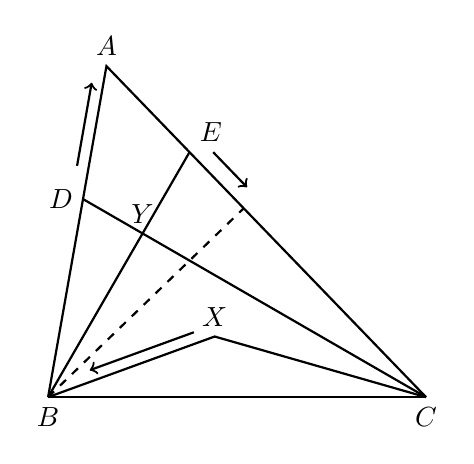
\begin{tikzpicture}[thick,scale=0.6]
\draw (0,0) node[below]{$B$} coordinate(B)--(8,0) node[below]{$C$} coordinate (C);
\path[name path=BX] (B)--(\xval:7);
\path[name path=BY] (B)--(\xval+\yval:7);
\path[name path=BA] (B)--(\xval+\xval+\yval:7.5);
\path[name path=CX] (C)--+(144+\xval:7);
\path[name path=CY] (C)--+(90+\xval+\yval:8.5);
\path[name path=CA] (C)--+(54+\xval+\xval+\yval:10);
\path[name intersections={of= BX and CX,by=X}];
\draw (B)--(X) node[above]{$X$}--(C);
\path[name intersections={of= BY and CY,by=Y}];
\path[name intersections={of= BA and CA,by=A}];
\draw (B)--(A)node[above]{$A$}--(C);
\path[name intersections={of= BY and CA,by=E}];
\path[name intersections={of= CY and BA,by=D}];
\draw (C)--(D)node[left]{$D$} (B)--(E)node[above right]{$E$};
\node[above] at (Y) {$Y$};
\path ( $(D)!.875!(A)$ )++(-.25,0) coordinate(R);
\draw[->] ( $(D)!.25!(A)$ )++(-.25,0)--(R);
\draw[dashed] (B)--( $(C)!(B)!(E)$ )coordinate (V);
\draw ( $(E)!.625!(V)$ )++(.5,0) coordinate (S);
\draw[->] (E)++(.5,0)--(S);
\path ( $(X)!.75!(B)$ )++(0,.25) coordinate(T);
\draw[->] ( $(X)!.125!(B)$ )++(0,.25)--(T);
\end{tikzpicture}
\end{document}
